\section{Summary and Conclusion}

\begin{frame}{Summary}
  \begin{enumerate}[\color{epflred}1.]
  \item<+-> a small set of chords is shared by many composers
  \item<+-> this core makes up large portions of their harmonic language
  \item<+-> important aspects of chord distributions are not yet well-understood
  \item<+-> the line of fifths can be retrieved from data
  \item<+-> using the \emph{Tonnetz} reveals stylistic differences
  \item<+-> both can be expanded from the study of single pieces to entire repertoires
\end{enumerate}
\end{frame}

\begin{frame}{Conclusion}
  \textbf{Computational Music Analysis}
  \begin{enumerate}[\color{epflred}1.]\pause
    \item<+-> forces precise definitions and models
    \item<+-> allows to test music theoretical concepts on large corpora
    \item<+-> facilitates interactions with other areas within and beyond musicology
    \item<+-> requires reflection, critique, and interpretation
  \end{enumerate}
\end{frame}

% \againframe<8->{disciplines}

% \begin{frame}{}
%   \begin{figure}
%     \centering
%     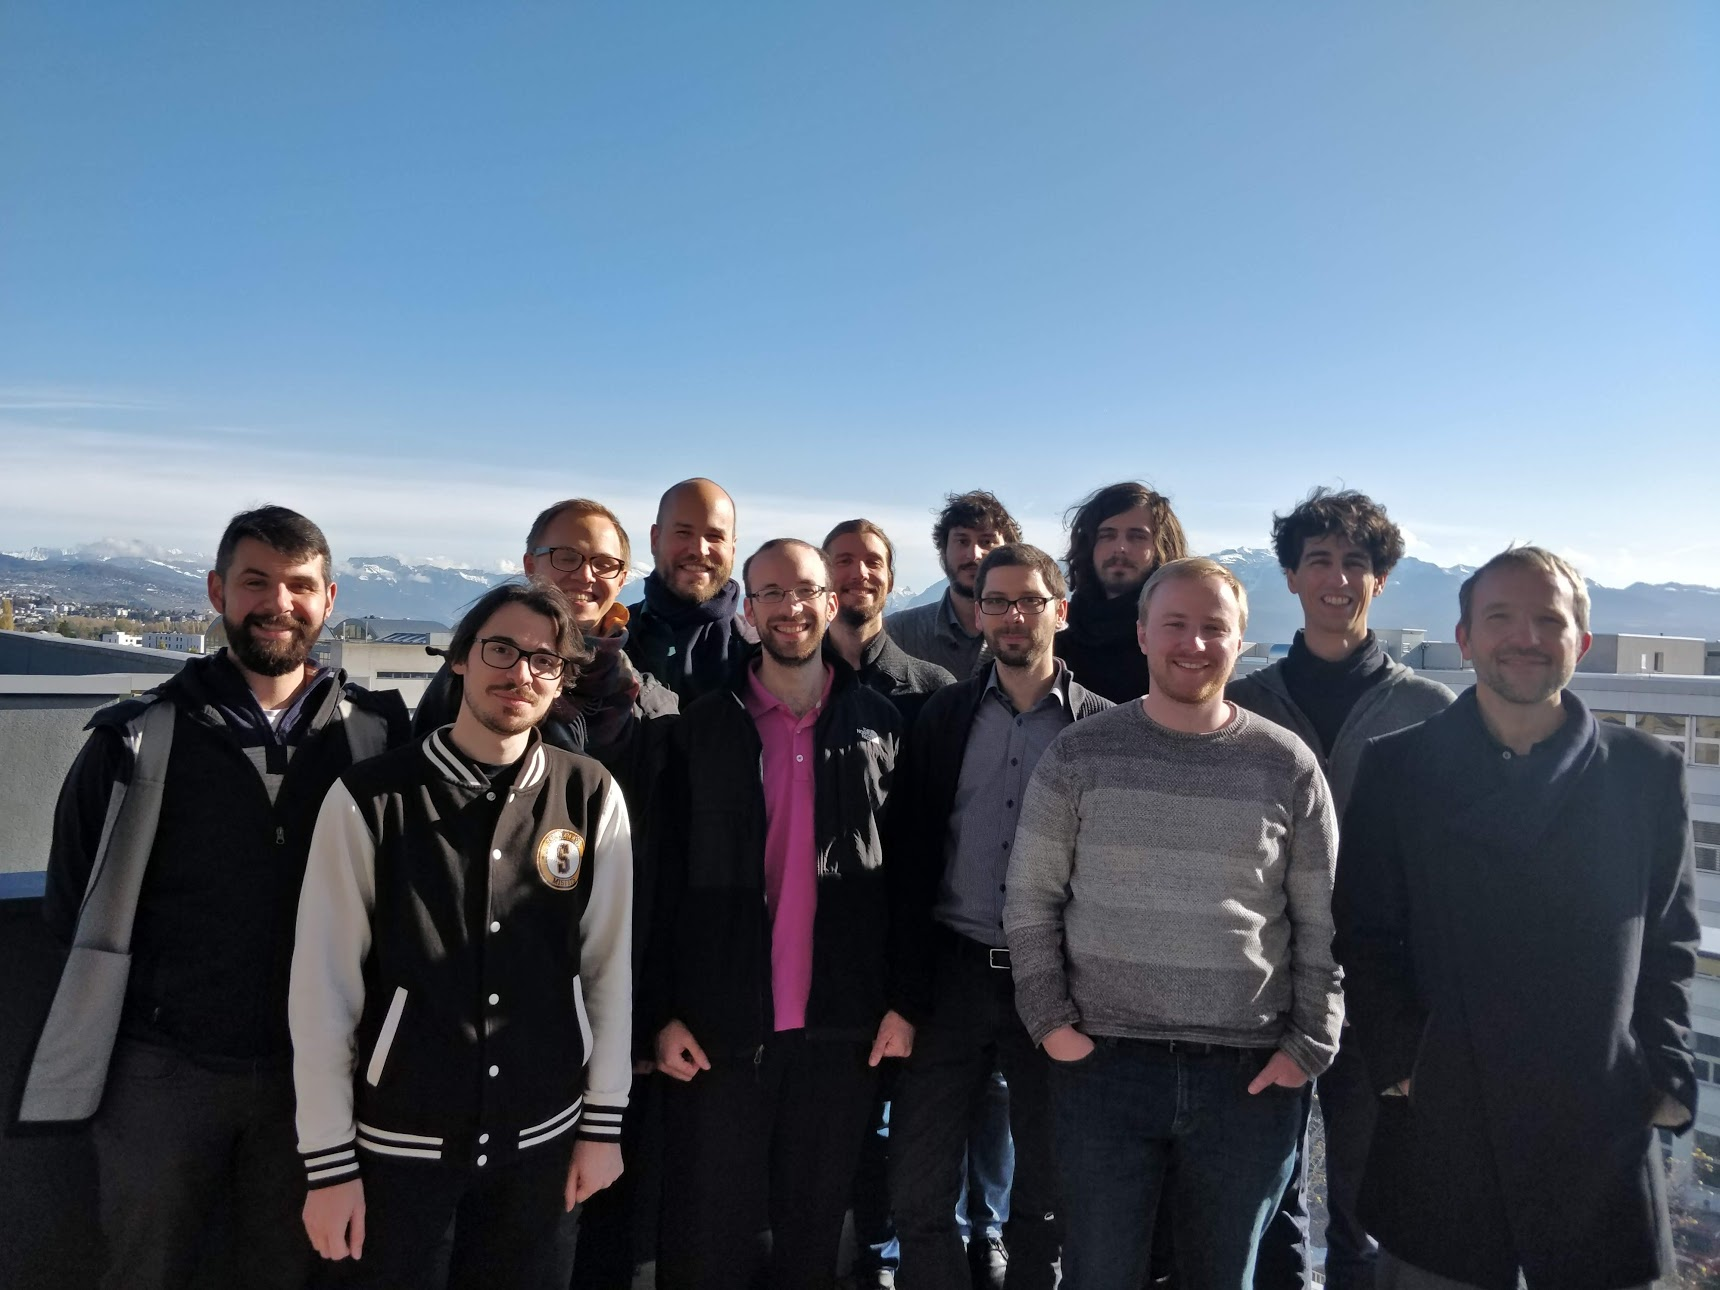
\includegraphics[height=.9\textheight]{img/dcml.jpg}
%     \caption*{Digital and Cognitive Musicology Lab, Lausanne, 2019}
%   \end{figure}
% \end{frame}

\begin{frame}[standout]
  Thank you very much!
\end{frame}
